\documentclass[11pt,aspectratio=169]{beamer}

\usepackage{slides}
\usepackage{soul}
\usepackage{pdfpc}
\usepackage{ebproof}
\usepackage{bigdelim}
\usepackage{booktabs}
\usepackage{listings}
\usepackage{tcolorbox}
\usepackage{tabularx}
\usepackage{tikz}
\usepackage{xspace}
\usepackage[T1]{fontenc}
\usepackage[utf8]{inputenc}
\usepackage[symbol]{footmisc}
\usepackage[noend]{algpseudocode}
\usepackage[
    backend    = biber,
    style      = alphabetic,
    giveninits = true,
    maxnames   = 16,
    minnames   = 16,
]{biblatex}

\addbibresource{./references.bib}

\usetikzlibrary{
    positioning,
    shapes.symbols,
    shadows,
    arrows,
    calc
}

\newcommand{\senc}{\text{senc}}
\newcommand{\msg}{\text{msg}}
\newcommand{\nonce}{\text{nonce}}
\newcommand{\KDF}{\text{KDF}}
\newcommand{\key}{\text{key}}

\newcommand{\Tamarin}[1]{\textsc{Tamarin}\xspace}

%% Print: [#1] -[#2]-> [#3]
\newcommand{\MSR}[3]{#1 -\hspace{-4pt}[\hspace{5pt} #2 \hspace{4pt}]\hspace{-4.6pt}\rightarrow #3}
%% Print: -[#1]->
\newcommand{\ActionFact}[1]{-\hspace{-4pt}[\hspace{5pt} #1 \hspace{4pt}]\hspace{-4.6pt}\rightarrow}
%% Print: ~
\newcommand{\tildelow}{\raisebox{0.5ex}{\texttildelow}}
%% Print: ^
\newcommand{\pow}{\textasciicircum{}}
%% Highlight text in overlay
\newcommand{\althl}[2][2]{\alt<#1>{\hl{#2}}{#2}}

%% Sticky notes to represent facts
\definecolor{StickyNoteYellow}{RGB}{241,239,161}
\definecolor{StickyNoteRed}{RGB}{255,167,169}
\definecolor{StickyNoteGreen}{RGB}{148,199,146}
\definecolor{StickyNoteBlue}{RGB}{167,229,241}
\NewDocumentCommand{\StickyNote}{O{StickyNoteYellow}O{1cm}m}{%
    \begin{tikzpicture}
        \node[
            drop shadow={
                shadow xshift = 2pt,
                shadow yshift = -4pt,
            },
            xslant = -0.1,
            yslant = 0.1,
            draw   = black,
            fill   = #1,
            text   = black,
        ] {\parbox[t][#2][c]{#2}{\centering#3}};
    \end{tikzpicture}
}

%% Colors for terms and facts
\definecolor{TermBlue}{HTML}{1C377D}
\definecolor{FactPurple}{HTML}{7C3655}

\newcommand{\term}[1]{\textcolor{TermBlue}{#1}}
\newcommand{\Term}[1]{\textcolor{TermBlue}{#1}}
\newcommand{\Fact}[1]{\textcolor{FactPurple}{#1}}

%% Other colors
\definecolor{AdversaryRed}{HTML}{DA3B26}

%% Listings
\lstset{escapeinside={(*@}{@*)}}
\lstset{numberstyle=\tiny}

\definecolor{TamarinBlue}{RGB}{42,0,255}
\definecolor{TamarinGreen}{RGB}{48,110,32}
\definecolor{TamarinPurple}{RGB}{175,36,67}

\lstdefinestyle{tamarin}{
    basicstyle    = \linespread{0.75}\footnotesize\ttfamily,
    extendedchars = true,
    tabsize       = 2,
    columns       = fixed,
    numbers       = none,
    breaklines    = true,
    literate      = {~}{{\raisebox{0.5ex}{\texttildelow}}}{1},
    morekeywords  = {theory, builtins, restriction, equations, functions, rule,
                     let, in, lemma, All, Ex, not, predicates, begin, end},
    keywordstyle  = \color{TamarinPurple},
    morecomment   = [l]{//},
    morecomment   = [s]{/*}{*/},
    commentstyle  = \color{TamarinGreen},
    xleftmargin   = 0mm,
    upquote       = true,
    morestring    = *[b]",
    showstringspaces = false
}

\lstdefinestyle{tactic}{
    basicstyle    = \linespread{0.75}\footnotesize\ttfamily,
    extendedchars = true,
    tabsize       = 2,
    columns       = fixed,
    numbers       = none,
    breaklines    = true,
    literate      = {~}{{\raisebox{0.5ex}{\texttildelow}}}{1},
    alsoletter    = :,
    morekeywords  = {tactic:, presort:, prio:, deprio:},
    keywordstyle  = \color{TamarinPurple},
    morecomment   = [l]{//},
    morecomment   = [s]{/*}{*/},
    commentstyle  = \color{TamarinGreen},
    xleftmargin   = 0mm,
    upquote       = true,
    morestring    = *[b]",
}

\lstdefinestyle{oracle}{
    basicstyle    = \linespread{0.75}\footnotesize\ttfamily,
    extendedchars = true,
    tabsize       = 2,
    columns       = fixed,
    numbers       = none,
    breaklines    = true,
    literate      = {~}{{\raisebox{0.5ex}{\texttildelow}}}{1},
    morecomment   = [l]{\#},
    morekeywords  = {import, for, in, if, elif},
    keywordstyle  = \color{TamarinPurple},
    commentstyle  = \color{TamarinGreen},
    xleftmargin   = 0mm,
    upquote       = true,
}

\definecolor{ProVerifGreen}{RGB}{48,110,32}
\definecolor{ProVerifBlue}{RGB}{64,112,161}

\lstdefinestyle{proverif}{
    basicstyle    = \linespread{0.75}\footnotesize\ttfamily,
    extendedchars = true,
    tabsize       = 2,
    columns       = fixed,
    numbers       = none,
    breaklines    = true,
    literate      = {~}{{\raisebox{0.5ex}{\texttildelow}}}{1},
    morecomment   = [s]{(*}{*)},
    commentstyle  = \color{ProVerifGreen},
    keywordstyle  = \color{ProVerifBlue},
    morekeywords  = {in, if, event, new, let, out},
    xleftmargin   = 0mm,
}

\definecolor{proofTreeBlue}{HTML}{2639B0}
\definecolor{proofTreeRed}{HTML}{921C12}

\lstdefinestyle{prooftree}{
    basicstyle    = \linespread{0.8}\footnotesize\fontfamily{pcr}\selectfont,
    extendedchars = true,
    tabsize       = 2,
    columns       = fixed,
    numbers       = left,
    breaklines    = true,
    literate      = {~}{{\raisebox{0.5ex}{\texttildelow}}}{1},
    keywords      = [1]{lemma, case, next, qed, by, end, Diff-Lemmas},
    keywordstyle  = [1]\color{black}\bfseries,
    keywords      = [2]{simplify, solve, sorry, contradiction, induction,
                        autoprove, rule-equivalence},
    keywordstyle  = [2]\color{proofTreeBlue}\bfseries,
    keywords      = [3]{@, \|, <, \^},
    keywordstyle  = [3]\color{proofTreeRed},
    alsoletter    = @\|<\^-,
    moredelim     = **[is][{\color{proofTreeBlue}}]{<<}{>>},
    xleftmargin   = 0mm,
    upquote       = true,
    morestring    = *[b]",
}

%% Color boxes
\definecolor{ColorBoxBlue}{HTML}{1C377D}
\tcbset{
    colback      = white,
    colframe     = black,
    fonttitle    = \bfseries,
    coltitle     = white,
    colbacktitle = ColorBoxBlue,
    boxrule      = 1pt
}

%% Vertical separator for frames
\newcommand<>{\vsep}{
    \begin{tikzpicture}[remember picture,overlay]%
        \draw[ultra thick]
            ($(current page.north west)+(8cm,0.5cm)$) to
            ($(current page.south west)+(8cm,-0.5cm)$)
        ;
    \end{tikzpicture}%
}

%% Horizontal separator for frames
\newcommand<>{\hsep}{
    \begin{tikzpicture}[remember picture,overlay]%
        \draw[ultra thick]
            ($(current page.north west)+(-0.5cm,-4.5cm)$) to
            ($(current page.north east)+(0.5cm,-4.5cm)$)
        ;
    \end{tikzpicture}%
}


\title{Formal Analysis of Real-World Security Protocols}
\subtitle{Lecture 1: Terms and Equational Theories}
\date{\today}
\author{Aleksi Peltonen}
\institute{CISPA Helmholtz Center for Information Security}

\begin{document}
\maketitle

% ---------------------------------------------------------------------------- %
% Content
% ---------------------------------------------------------------------------- %

\begin{frame}[fragile]{Recap: protocol verification}
    \begin{figure}
        \centering
        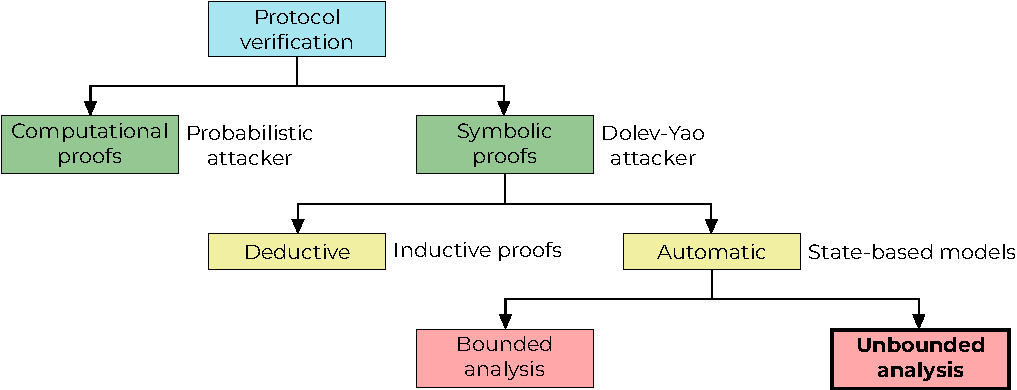
\includegraphics[width=\textwidth]
            {figures/lecture_1/protocol_verification}
    \end{figure}
\end{frame}

\begin{frame}[fragile]{Recap: formal verification}
    Recall our goals:
    \begin{itemize}
        \item We want to \textbf{formally analyze (real-world) protocols}
        \item Find attacks, or prove that protocols are ``secure''
    \end{itemize}
    To achieve this, we plan to:
    \begin{itemize}
        \item Capture all possible interactions between the protocol and an 
              attacker in a mathematical model $\mathrm{M}$
        \item Formally state our desired security goal $\varphi$ in terms of 
              this model
        \item Then, either \textbf{prove that $\mathrm{M} \vDash \varphi$} or 
              \textbf{find a counterexample} that shows
              $\neg (\mathrm{M} \vDash \varphi$) (i.e., an attack)
    \end{itemize}
    The models are complex, but designed with \textbf{automation} in mind
\end{frame}

\begin{frame}[fragile]{Model components}
    What \textbf{components} do we need to model protocols?
    \begin{table}
        \raggedright
        \begin{tabular}{lll}
            1. & All possible sent and received messages
               & \rdelim\}{1}{3mm}[\hspace*{3mm}\hl{Lecture 1}] \\[.2cm]
            2. & All possible protocol behaviors
               & \rdelim\}{1}{3mm}[\hspace*{3mm}Lecture 2] \\[.2cm]
            3. & The attacker
               & \rdelim\}{2.2}{3mm}[\hspace*{2mm}Lecture 3] \\[.2cm]
            4. & Security properties that we want to verify
        \end{tabular}
    \end{table}
\end{frame}

\begin{frame}[fragile]{This lecture}
    \tableofcontents
\end{frame}

% ---------------------------------------------------------------------------- %

\section{Modeling Messages as Terms}

% ---------------------------------------------------------------------------- %

\begin{frame}[fragile]{Messages}
    \begin{columns}
        \begin{column}{0.5\textwidth}
            \begin{itemize}
                \item In reality, protocols send and receive \textbf{bitstrings}
                \item We can model this... but we don't know how to
                      \textbf{automate} the resulting analysis
                \item Observation: maybe we don't care about all bitstrings, 
                      only some are relevant
                \item Choice: \textbf{focus on how the bits were computed}, not 
                      on values
            \end{itemize}
        \end{column}
        \vsep
        \begin{column}{0.5\textwidth}
            \footnotesize\textit{
                Alice is expecting a message containing her name, a new random 
                value, and a signature with Bob's private key. Which messages 
                would Alice accept?
            }
            \begin{figure}
                \vspace*{.4cm}
                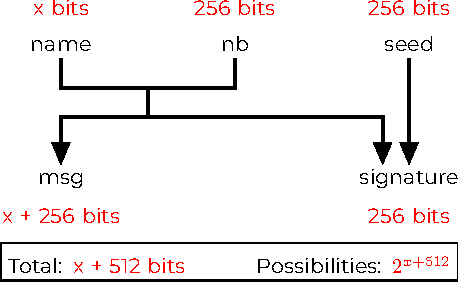
\includegraphics[width=.8\textwidth]
                    {./figures/lecture_1/signature_example}
                \vspace*{-.4cm}
            \end{figure}
        \end{column}
    \end{columns}
\end{frame}

\begin{frame}[fragile]{Messages}
    \textbf{\textit{Very} informal intuition}
    \begin{itemize}
        \item If someone generates a new large random value, we do not care 
              about the actual bits, only that it is ``fresh'' and is unlikely 
              to match any other bitstrings we have seen
        \item The only way anyone can find the bitstring \verb|hash(`Dog')| is 
              by being incredibly lucky, or by computing this hash themselves 
              from the string \verb|`Dog'|
              \textbf{We omit luck from our model!}
        \item Similarly for encryptions and signatures: outputs look like 
              random bits; negligible chance to coincide with other computed 
              values
    \end{itemize}
\end{frame}

\begin{frame}[fragile]{Signatures}
    A \textbf{signature} describes the non-logical symbols of a formal language.
    \\[.3cm]
    Formally, a signature $\Sigma$ is a set of \textbf{function symbols} and a 
    function $Ar: \Sigma \rightarrow \mathbb{N}$. Function symbols of arity 0 
    are called \textbf{constants}.

    \begin{tcolorbox}[title=Example]
        $\Sigma = \{Alice, Bob, Charlie, hash, pair, exp\}$, where $Alice$, 
        $Bob$, and $Charlie$ are constants (i.e., $Ar(Alice) = Ar(Bob) = Ar
        (Charlie) = 0$), and $hash$, $pair$, $exp$ are functions with
        $Ar(hash) = 1$ and $Ar(pair) = Ar(exp) = 2$
    \end{tcolorbox}
\end{frame}

\begin{frame}[fragile]{Terms}
    A \textbf{term} is recursively constructed from constants, variables, and 
    function symbols.

    \begin{tcolorbox}[title=Example]
        t = $(x + y) \times (1 + z)$ is a term built from the constant $1$, 
        variables $x$, $y$, and $z$, and the function symbols $+$ and $\times$
    \end{tcolorbox}

    Let $\Sigma$ be a signature, $\mathcal{V}$ a set of variables,  and 
    $\mathcal{C}$ a set of constants. We call the set $\mathcal{T}_{\Sigma}
    (\mathcal{V} \cup \mathcal{C})$ the \textbf{term algebra} over $\Sigma$.
    \\[.3cm]
    We can use terms to \textit{represent messages!}
\end{frame}

\begin{frame}[fragile]{Modeling messages as terms}
    \textbf{Terms} represent messages by the way they were constructed.
    \begin{table}[]
        \raggedright
        \begin{tabular}{@{}ll}
            \textbf{Basic terms:}
              & \textcolor{TermBlue}{
                    Alice, Bob, x, y, z, ServerNonce, `some\_string'}\\[.3cm]
            \textbf{Function symbols}: 
              & \textcolor{TermBlue}{pair/2, exp/2, hash/1, sign/2, verify/3}\\
              & \textcolor{TermBlue}{senc/2, sdec/2} \\
        \end{tabular}
    \end{table}

    We often use common shorthands in tools and writing:
    \begin{table}[]
        \begin{tabular}{lll}
            \textcolor{TermBlue}{<x, y>} & for
                & \textcolor{TermBlue}{pair(x, y)} \\
            \textcolor{TermBlue}{<x, y, z>} & for
                & \textcolor{TermBlue}{pair(pair(x, y), z)} \\
            \textcolor{TermBlue}{x\pow{}y} & for
                & \textcolor{TermBlue}{exp(x, y)} \\
        \end{tabular}
    \end{table}
\end{frame}

\begin{frame}[fragile]{Terms are trees}
    \textcolor{TermBlue}{senc( <'Message1', NewKey, Bob>,
        KDF( <MasterKey, Alice, Bob> ) )}
    \begin{figure}
        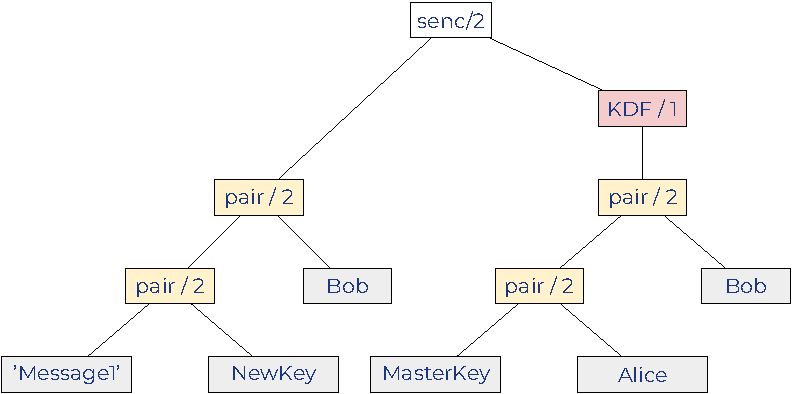
\includegraphics[width=.8\textwidth]
            {figures/lecture_1/terms_1}
    \end{figure}
\end{frame}

\begin{frame}[fragile]{Variables and types}
    \begin{itemize}
        \item Terms can contain \textbf{variables}
              (e.g., \textcolor{TermBlue}{hash(X)})
        \item Variables can have \textit{type annotations} that restrict the 
              possible values that they can be instantiated with:
        \begin{itemize}
            \item \textcolor{TermBlue}{\phantom{\tildelow}X} is a variable 
                  without type annotation
            \item \textcolor{TermBlue}{\tildelow{}X} is a \textit{fresh} 
                  variable that can only be instantiated with randomly 
                  generated values
            \item \textcolor{TermBlue}{\$X} is a public variable that can only 
                  be instantiated with values that are known to all parties
        \end{itemize}
        \item We use terms to..
        \begin{itemize}
            \item ..construct \textbf{sent and received messages} according to 
                  a protocol specification
            \item ..determine the \textbf{attacker's knowledge}: Which terms 
                  does the attacker know? Which terms can the attacker 
                  construct?
        \end{itemize}
    \end{itemize}
\end{frame}

\begin{frame}[fragile]{Example: Basic attacker derivation}
    \begin{itemize}
        \item Assume that the attacker starts out knowing all public 
              information:
        \begin{itemize}
            \item Public constants, text strings, public variables:
            \begin{itemize}
                \item \textcolor{TermBlue}{Alice, Bob, `alice', `bob',
                      \tildelow{}nonce, \$identifier, $\dots$}
            \end{itemize}
            \item Algorithms:
            \begin{itemize}
                \item \textcolor{TermBlue}{senc, sdec, hash, KDF, $\dots$}
            \end{itemize}
        \end{itemize}
        \item The attacker can generate new fresh values
        \item From the known values, the attacker can compute e.g.,
        \begin{itemize}
            \item \textcolor{TermBlue}{
                senc(hash(<Alice, `alice'>), KDF(~AttackerKey))}
        \end{itemize}
        \item After learning a fresh term \textcolor{TermBlue}{NonceBob} from a 
              message, the attacker can also compute e.g.,
        \begin{itemize}
            \item \textcolor{TermBlue}{
                senc(hash(<Bob, NonceBob>), KDF(~AttackerKey))}
        \end{itemize}
    \end{itemize}
\end{frame}

\begin{frame}[fragile]{Syntactic equality}
    \begin{itemize}
        \item \textbf{Syntactic equality:} two terms are the same, if and only 
              if they are syntactically equivalent
        \item We decided earlier that the outputs of cryptographic primitives 
              are supposed to look random. Syntactic equality encodes this intuition

        \begin{tabular}{lcll}
            & & & \\
              \textcolor{TermBlue}{`dog'}
            & \textcolor{TermBlue}{=}
            & \textcolor{TermBlue}{`dog'}
            & \\
              \textcolor{TermBlue}{`dog'}
            & \textcolor{TermBlue}{$\neq$}
            & \textcolor{TermBlue}{hash(X)}
            & for all \textcolor{TermBlue}{X}\\
              \textcolor{TermBlue}{hash(X)}
            & \textcolor{TermBlue}{=}
            & \textcolor{TermBlue}{hash(Y)}
            & if and only if \textcolor{TermBlue}{X = Y}\\
              \textcolor{TermBlue}{senc(m1, k1)}
            & \textcolor{TermBlue}{=}
            & \textcolor{TermBlue}{senc(m2, k2)}
            & if and only if \textcolor{TermBlue}{m1 = m2} and
              \textcolor{TermBlue}{k1 = k2}\\
              \textcolor{TermBlue}{senc(m, k)}
            & \textcolor{TermBlue}{$\neq$}
            & \textcolor{TermBlue}{hash(X)}
            & for all \textcolor{TermBlue}{m, k, X}\\
        \end{tabular}    
    \end{itemize}
\end{frame}

\begin{frame}[fragile]{Example: Diffie-Hellman key exchange}
    Now, with a more formal syntax for messages, we can revisit our example 
    from the previous lecture.
    \begin{figure}
        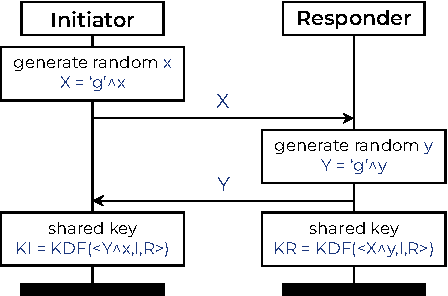
\includegraphics[width=.5\textwidth]{./figures/lecture_1/dh}
    \end{figure}
\end{frame}

\begin{frame}[fragile]{Normal execution: key is secret}
    \begin{itemize}
        \item In a normal execution, \textcolor{TermBlue}{x $\neq$ y} (i.e., 
              both are freshly generated)
        \begin{itemize}
            \item The initiator derives \textcolor{TermBlue}{KI = KDF(Y\pow{}x)}
            \item The responder derives \textcolor{TermBlue}{KR = KDF(X\pow{}y)}
        \end{itemize}
        \item The (network) attacker knows
        \begin{itemize}
            \item \textcolor{TermBlue}{X = `g'\pow{}x}
            \item \textcolor{TermBlue}{Y = `g'\pow{}y}
        \end{itemize}
        \item ..but has no way to construct KI or KR without knowing
        \begin{itemize}
            \item \textcolor{TermBlue}{X\pow{}y = (`g'\pow{}x)\pow{}y}, or
                  \textcolor{TermBlue}{Y\pow{}x = (`g'\pow{}y)\pow{}x}
        \end{itemize}
        \item ..which it cannot, since there is no way to extract
              \textcolor{TermBlue}{x} or \textcolor{TermBlue}{y}
        \item This corresponds to the \textit{hardness of the discrete 
              logarithm problem}
    \end{itemize}
\end{frame}

\begin{frame}[fragile]{Exponentiation as expected?}
    \begin{itemize}
        \item In a normal execution, \textcolor{TermBlue}{x $\neq$ y}
              (i.e., both are freshly generated)
        \begin{itemize}
            \item The initiator derives \textcolor{TermBlue}{KI = KDF(Y\pow{}x)}
            \item The responder derives \textcolor{TermBlue}{KR = KDF(X\pow{}y)}
        \end{itemize}
        \item By syntactic equality:
        \begin{itemize}
            \item \textcolor{TermBlue}{KI = KR} if and only if
            \textcolor{TermBlue}{(`g'\pow{}y)\pow{}x = (`g'\pow{}x)\pow{}y}
        \end{itemize}
        \item Since \textcolor{TermBlue}{x $\neq$ y}, \textit{this never holds}
        \item Thus, in normal execution of this model, \textbf{the initiator 
              and the responder compute different, non-equal terms}
        \item We need something else to fix this
    \end{itemize}
\end{frame}

% ---------------------------------------------------------------------------- %

\section{Equational Theories}

% ---------------------------------------------------------------------------- %

\begin{frame}[fragile]{Equational theories}
    An \textbf{equational theory} is a set of rules that determine which terms 
    are considered equivalent.

    Motivation:
    \begin{itemize}
        \item Some messages (such as exponentiation) can be constructed in more 
              than one way
        \item Convenient modeling for cryptographic primitives
        \item Allows us to model degenerate cases of cryptographic primitives
    \end{itemize}
\end{frame}

\begin{frame}[fragile]{Equational theories}
    \textbf{Definitions:}
    \begin{itemize}
        \item An \textbf{equation} over the signature $\Sigma$ is a pair of 
              terms $s,t \in \mathcal{T}_{\Sigma}(\mathcal{V})$ that defines 
              when the terms are considered equal
        \begin{itemize}
            \item For example, instead of modeling exponentiation, we use an 
                  equation to define the expected equality:
                  \textcolor{TermBlue}{(X\pow{}Y)\pow{}Z = (X\pow{}Z)\pow{}Y}
            \item ...which implies \textcolor{TermBlue}{
                  (`g'\pow{}y)\pow{}x = (`g'\pow{}x)\pow{}y}
        \end{itemize}
        \item An \textbf{equational theory} is a tuple $(\Sigma, E)$ of a 
              signature $\Sigma$ and a set of equations $E$
    \end{itemize}
\end{frame}

\begin{frame}[fragile]{Pairing}
    For pairing, we use an equational theory to model splitting pairs.\\[.3cm]

    \textbf{Functions symbols:}
    \begin{table}[]
        \raggedright
        \begin{tabular}{ll}
            \textcolor{TermBlue}{pair/2}
            & pair two terms
                (\textcolor{TermBlue}{pair(x, y)} is often written as
                \textcolor{TermBlue}{<x, y>}) \\
            \textcolor{TermBlue}{fst/1}
            & extract the first element from a pair \\
            \textcolor{TermBlue}{snd/1}
            & extract the second element from a pair
        \end{tabular}
    \end{table}

    \textbf{Equational theory:}
    \begin{table}[]
        \raggedright
        {\color{TermBlue}
        \begin{tabular}{lll}
            fst( <x, y> ) & = & x \\
            snd( <x, y> ) & = & y
        \end{tabular}}
    \end{table}
\end{frame}

% ---------------------------------------------------------------------------- %

\section{Equational Theories for Cryptographic Primitives}

% ---------------------------------------------------------------------------- %

\begin{frame}[fragile]{Tamarin's built-in equational theories}
    \begin{table}[]
        \vspace*{-.2cm}
        \begin{tabular}{lll}
            \toprule
            \textbf{Name} & \textbf{Description} \\
            \midrule
                \verb|hashing|
                    & Defines a hash function \verb|h| \\
                \verb|asymmetric-encryption|
                    & \althl{Asymmetric encryption} \\
                \verb|symmetric-encryption|
                    & \althl{Symmetric encryption} \\
                \verb|signing|
                    & \althl{Basic signatures} \\
                \verb|revealing-signing|
                    & Signatures that allow plaintext extraction \\
                \verb|multiset|
                    & Multisets (bags) in messages \\
                \verb|xor|
                    & \althl{Exclusive-or} \\
                \verb|diffie-hellman|
                    & \althl{Diffie-Hellman style exponentiation} \\
                \verb|bilinear-pairing|
                    & Bilinear pairing \\
                \verb|natural numbers|
                    & Natural numbers and counters \\
            \bottomrule
        \end{tabular}
    \end{table}
\end{frame}

\begin{frame}[fragile]{Basic symmetric encryption}
    For basic symmetric encryption schemes, we use an equational theory to 
    model decryption.\\[.3cm]

    \textbf{Functions symbols:}
    \begin{table}[]
        \raggedright
        \begin{tabular}{ll}
            \textcolor{TermBlue}{senc/2} & encrypt a message using a key \\
            \textcolor{TermBlue}{sdec/2} & decrypt a message using a key
        \end{tabular}
    \end{table}

    \textbf{Equational theory:}
    \begin{table}[]
        \raggedright
        {\color{TermBlue}
        \begin{tabular}{l}
            sdec(senc(m, k), k) = m
        \end{tabular}}
    \end{table}
\end{frame}

\begin{frame}[fragile]{Basic asymmetric encryption}
    For basic asymmetric encryption schemes, where the public key can be 
    computed from the private key, we use an equational theory to model 
    decryption.\\[.3cm]

    \textbf{Functions symbols:}
    \begin{table}[]
        \raggedright
        \begin{tabular}{ll}
            \textcolor{TermBlue}{aenc/2}
                & encrypt a message using a public key \\
            \textcolor{TermBlue}{adec/2}
                & decrypt a message using the private key \\
            \textcolor{TermBlue}{pk/1}
                & compute the public key from a private key
        \end{tabular}
    \end{table}

    \textbf{Equational theory:}
    \begin{table}[]
        \raggedright
        {\color{TermBlue}
        \begin{tabular}{l}
            adec(aenc(m, pk(sk)), sk) = m
        \end{tabular}}
    \end{table}
\end{frame}

\begin{frame}[fragile]{Basic signature scheme}
    For basic signature schemes, we use an equational theory to model signature 
    verification.\\[.3cm]

    \textbf{Functions symbols:}
    \begin{table}[]
        \raggedright
        \begin{tabular}{ll}
            \textcolor{TermBlue}{sign/2}
                & sign a message with a (private) signing key \\
            \textcolor{TermBlue}{verify/3}
                & verify a signature for a message and a verification key \\
            \textcolor{TermBlue}{pk/1}
                & compute the verification key from signing key \\
            \textcolor{TermBlue}{true}
                & a constant representing `true'
        \end{tabular}
    \end{table}

    \textbf{Equational theory:}
    \begin{table}[]
        \raggedright
        {\color{TermBlue}
        \begin{tabular}{l}
            verify(sign(m, sk), m, pk(sk)) = true
        \end{tabular}}
    \end{table}
\end{frame}

\begin{frame}[fragile]{Diffie-Hellman}
    Diffie-Hellman modular exponentiation is a complex example.\\[.3cm]

    \textbf{Functions symbols:}
    \begin{table}[]
        \raggedright
        \begin{tabular}{ll}
            \textcolor{TermBlue}{\pow}
                & exponentiation in the group (modulo some large prime) \\
            \textcolor{TermBlue}{*}
                & multiplication \\
            \textcolor{TermBlue}{inv/1}
                & inverse \\
            \textcolor{TermBlue}{1}
                & a constant representing `1'
        \end{tabular}
    \end{table}

    \textbf{Equational theory:}
    \begin{table}[]
        \raggedright
        {\color{TermBlue}
        \begin{tabular}{ll @{\hskip .8in} ll @{\hskip .8in} ll}
            (x \pow y) \pow z & = x \pow (y * z)
           & x \pow 1         & = x
           & x * y            & = y * x \\ 
            (x * y) * z       & = x * (y * z)
           & x * 1            & = x
           & x * inv(x)       & = 1
        \end{tabular}}
    \end{table}
\end{frame}

\begin{frame}[fragile]{Exclusive-or}
    \textbf{Functions symbols:}
    \begin{table}[]
        \raggedright
        \begin{tabular}{ll}
            \textcolor{TermBlue}{$\oplus$} & exclusive-or of two terms \\
            \textcolor{TermBlue}{zero}
                & a constant representing an all-zeroes bitstring \\
        \end{tabular}
    \end{table}

    \textbf{Equational theory:}
    \begin{table}[]
        \raggedright
        {\color{TermBlue}
        \begin{tabular}{ll @{\hskip .8in} ll}
             x $\oplus$ y & = y $\oplus$ x &
            (x $\oplus$ y) $\oplus$ z & = x $\oplus$ (y $\oplus$ z) \\
             x $\oplus$ zero & = x &
             x $\oplus$ x & = zero
        \end{tabular}}
    \end{table}

    \textbf{Note:} this is a very coarse approximation of xor that does not 
        work well with other primitives and needs to be handled with care.
\end{frame}

\begin{frame}[fragile]{Further primitives}
    \begin{itemize}
        \item \textbf{The previous were only basic examples} corresponding to 
              some of Tamarin's built-in schemes
        \item Tamarin (and other symbolic tools) can handle many more 
              primitives, such as
        \begin{itemize}
            \item Multisets, blind signatures, bilinear pairings, $\dots$
        \end{itemize}
        \item We can also provide much more accurate model of various different 
              signature schemes, Diffie-Hellman groups, or elliptic curves, etc.
        \item \textbf{We will return to user-specified equational theories 
                      later in the course!}
    \end{itemize}
\end{frame}

% ---------------------------------------------------------------------------- %

\section{Term Rewriting}

% ---------------------------------------------------------------------------- %

\begin{frame}[fragile]{Positions}
    \begin{itemize}
        \item Recall from earlier that terms are structured as \textit{trees}
        \item Each node in the tree has a unique \textbf{position} (think path) 
              indicating its place in the tree
        \item A position $p$ is a sequence of natural numbers\par
    \end{itemize}
    \vfill
    \begin{center}
        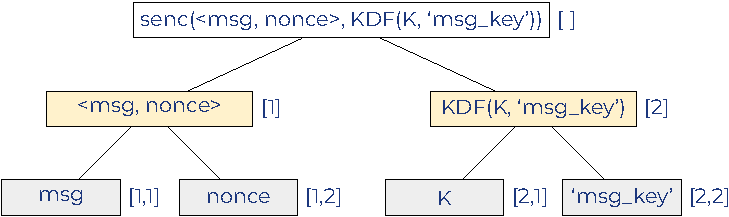
\includegraphics[width=.6\textwidth]{figures/lecture_1/terms_2}
    \end{center}
\end{frame}

\begin{frame}[fragile]{Subterms}
    \begin{itemize}
        \item Each position $p$ of a term $t$ is the start of a unique
              \textbf{subterm} $t|_p$
        \begin{table}[]
            \footnotesize
            \raggedright
            \begin{tabular}{p{0.08\textwidth}p{0.02\textwidth}p{0.7\textwidth}}
                $t|_{[]}$    & $=$
                    & $\senc(<\msg, \nonce>, \KDF(K,$`$\msg\_\key$'$))$\\
                $t|_{[1]}$   & $=$ & $<\msg, \nonce>$\\
                $t|_{[2]}$   & $=$ & $\KDF(\text{K}, $`$\msg\_\key$'$)$\\
                $t|_{[1,1]}$ & $=$ & $\msg$\\
                $t|_{[1,2]}$ & $=$ & $\nonce$\\
                $t|_{[2,1]}$ & $=$ & $\text{K}$\\
                $t|_{[2,2]}$ & $=$ & `$\msg\_\key$'
            \end{tabular}
        \end{table}
    \end{itemize}
    \vfill
    \begin{center}
        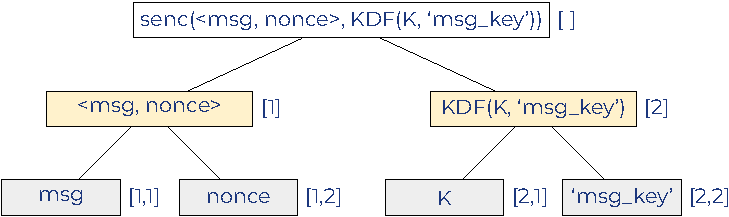
\includegraphics[width=.6\textwidth]{figures/lecture_1/terms_2}
    \end{center}
\end{frame}

\begin{frame}[fragile]{Substitutions}
    A \textbf{substitution} is a mapping $\sigma: \mathcal{V} \rightarrow 
    \mathcal{T}$ from variables to terms.\\[.3cm]

    We write $t\sigma$ to denote applying the substitution $\sigma$ to the term 
    $t$.\\[.3cm]

    This replaces each variable $x$ in $t$ by the term $x\sigma$.\\[.3cm]

    \begin{tcolorbox}[title=Example]
        For $t = \senc(<\msg, \nonce>, x)$ and
        $\sigma = \{x \mapsto \KDF(K,$`$\msg\_\key$'$)\}$,
        we can apply the substitution
        $x\sigma = \KDF(K,$`$\msg\_\key$'$)$
        to get
        $t\sigma = \senc(<\msg, \nonce>, \KDF(K, $`$\msg\_\key$'$))$.
    \end{tcolorbox}
\end{frame}

\begin{frame}[fragile]{Unification and matching}
    \textbf{Unification} determines if two terms with variables can be made 
    equal. Two terms $u$ and $v$ are said \textit{unifiable} if there exists a 
    substitution $\sigma$, called a \textit{unifier}, such that
    $u\sigma = v\sigma$.

    \begin{tcolorbox}[title=Example]
        The terms $t_1 = x$ and $t_2 = 2y$ are unifiable with e.g.,
        $\sigma = \{x \mapsto 2, y \mapsto 1\}$
    \end{tcolorbox}

    A term $t_1$ \textbf{matches} another term $t_2$ if there is a substitution 
    $\sigma$ s.t. $t_1 = t_2\sigma$

    \begin{tcolorbox}[title=Example]
        The term $t_1 = 1$ matches the term $t_2 = y$ with
        $\sigma = \{y \mapsto 1\}$
    \end{tcolorbox}
\end{frame}

\begin{frame}[fragile]{Term rewriting}
    \begin{itemize}
        \item A \textbf{rewrite rule} $l \rightarrow r$ over a signature 
              $\Sigma$ is an ordered pair of terms $(l, r)$ with
              $l,r \in \mathcal{T}_{\Sigma}(\mathcal{V})$
        \begin{itemize}
            \item Indicates that the left-hand side $l$ can be replaced by the 
                  right-hand side $r$
            \item Can be applied to a term $s$ if the left term $l$ matches 
                  some subterm of $s$, i.e., there is some substitution 
                  $\sigma$ s.t., the subterm of $s$ at position $p$ is the 
                  result of applying $\sigma$ to $l$
        \end{itemize}
        \item The outcome is the result of replacing the subterm at position 
              $p$ in $s$ by the term $r$ with the substitution $\sigma$ applied
        \item A \textbf{rewrite system} $\mathcal{R}$ is a set of rewrite rules
    \end{itemize}
\end{frame}

\begin{frame}[fragile]{Term rewriting example}
    \begin{tcolorbox}[title=Example]
        The \textit{distributive property} of binary operations is a rewriting 
        rule, which states that $x \times (y + z) \rightarrow x \times y + x 
        \times z$. Consider the term $s = a \times (b + 1)$ and the 
        substitution $\sigma = \{x \mapsto a, y \mapsto b, z \mapsto 1\}$. We 
        can apply the substitution $\sigma$ and the rewrite rule $l \rightarrow 
        r$ to obtain $t = a \times (b + 1) = a \times b + a \times 1 = a \times 
        b + a$.
    \end{tcolorbox}
\end{frame}

% ---------------------------------------------------------------------------- %

\section*{Summary}

% ---------------------------------------------------------------------------- %

\begin{frame}[fragile]{Summary}
    \begin{itemize}
        \item We have now learned that..
        \begin{itemize}
            \item \textbf{terms} can be used to represent messages,
            \item \textbf{equations} specify when two terms are considered 
                  equal, and
            \item \textbf{term rewriting rules} can be used to replace terms 
                  with other terms.
        \end{itemize}
        \item Why is this important?
        \begin{itemize}
            \item Tamarin models protocols as
                  \textbf{multiset rewriting rules with equations}
            \item We can model messages as ground terms!
        \end{itemize}
        \item In the next lecture, we will learn about modeling states as 
              \textbf{multisets of facts} and protocol executions as a
              \textbf{transition system} operating on them
    \end{itemize}
\end{frame}

% ---------------------------------------------------------------------------- %
% Reading Material
% ---------------------------------------------------------------------------- %
\begin{frame}[fragile]{Reading material}
    \textbf{Recommended reading}:\\ \;
        ~\cite[Ch. 3--3.1.4, 7]{tamarin-book},
        ~\cite[Ch. 2]{meier2013thesis}
    \begin{refsection}
        \nocite{tamarin-book, meier2013thesis}
        \printbibliography[heading=none]
    \end{refsection}
\end{frame}

\begin{frame}[fragile]{Additional reading}
    \textbf{Additional reading}:
        ~\cite[Ch. 2, 10--11]{baader1998terms},
        ~\cite{dreier2018xor}
    \begin{refsection}
        \nocite{dreier2018xor, baader1998terms}
        \printbibliography[heading=none]
    \end{refsection}
\end{frame}
% ---------------------------------------------------------------------------- %

\end{document}
